\documentclass[12pt]{article}
\usepackage{amsmath}
\usepackage{tikz}
\usepackage{pgfplots}
\pgfplotsset{compat=1.18}

\begin{document}

\title{\begin{Huge}{Linear Equations:}\end{Huge}\\Lengths, Midpoints,\\Perpendicular Lines,\\\& Intersection Points}\\
\author{Tutoring Centre Ferndale\\
\includegraphics[width=4em]{ApS_logo.png}}
\date{}
\maketitle

\newpage

\section*{Finding the Length of a Line Segment}

Using Pythagoras' formula for the lengths of the hypotenuse of a right triangle, the length of a line segment with endpoints \((x_1, y_1)\) and \((x_2, y_2)\) is given by the distance formula:
\[
d = \sqrt{(x_2 - x_1)^2 + (y_2 - y_1)^2}
\]

\subsection*{Example}

Find the length of the line segment with endpoints \((1, 2)\) and \((4, 6)\).

\[
d = \sqrt{(4 - 1)^2 + (6 - 2)^2} = \sqrt{3^2 + 4^2} = \sqrt{9 + 16} = \sqrt{25} = 5
\]\\

\begin{center}
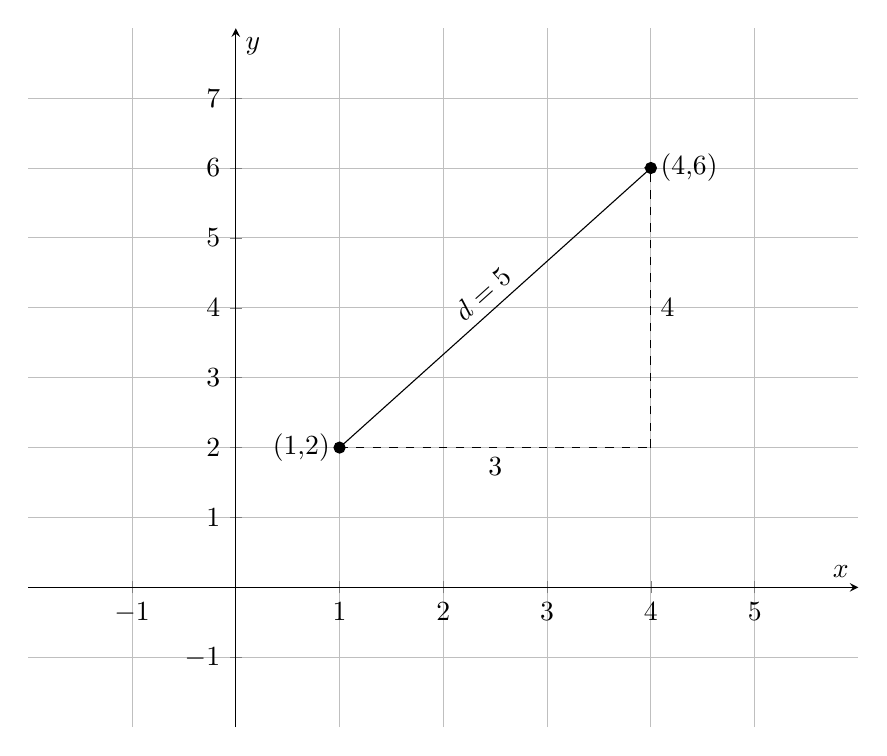
\begin{tikzpicture}
    \begin{axis}[width=\textwidth,
        axis lines = middle,
        xlabel = {$x$},
        ylabel = {$y$},
        ymin=-2, ymax=8,
        xmin=-2, xmax=6,
        ytick={-1,0,1,2,3,4,5,6,7},
        xtick={-1,0,1,2,3,4,5},
        grid=both,
        grid style={line width=.3pt, draw=gray!50}]
    \addplot [only marks, mark=*] coordinates {(1,2) (4,6)};
    \draw[->] (axis cs:1,2) -- (axis cs:4,6) node[midway,sloped,above]{$d=5$};
    \node at (axis cs:1,2) [anchor=east] {(1,2)};
    \node at (axis cs:4,6) [anchor=west] {(4,6)};
    \draw[dashed] (axis cs:1,2) -- (axis cs:4,2);
    \draw[dashed] (axis cs:4,2) -- (axis cs:4,6);
    \node at (axis cs:2.5,2) [anchor=north] {$3$};
    \node at (axis cs:4,4) [anchor=west] {$4$};
    \end{axis}
\end{tikzpicture}
\end{center}

\newpage

\section*{Finding the Midpoint of a Line Segment}

The midpoint of a line segment with endpoints \((x_1, y_1)\) and \((x_2, y_2)\) is given by:
\[
\left( \frac{x_1 + x_2}{2}, \frac{y_1 + y_2}{2} \right)
\]

\subsection*{Example}

Find the midpoint of the line segment with endpoints \((2, 3)\) and \((4, 7)\).

\[
\left( \frac{2 + 4}{2}, \frac{3 + 7}{2} \right) = (3, 5)
\]\\

\begin{center}
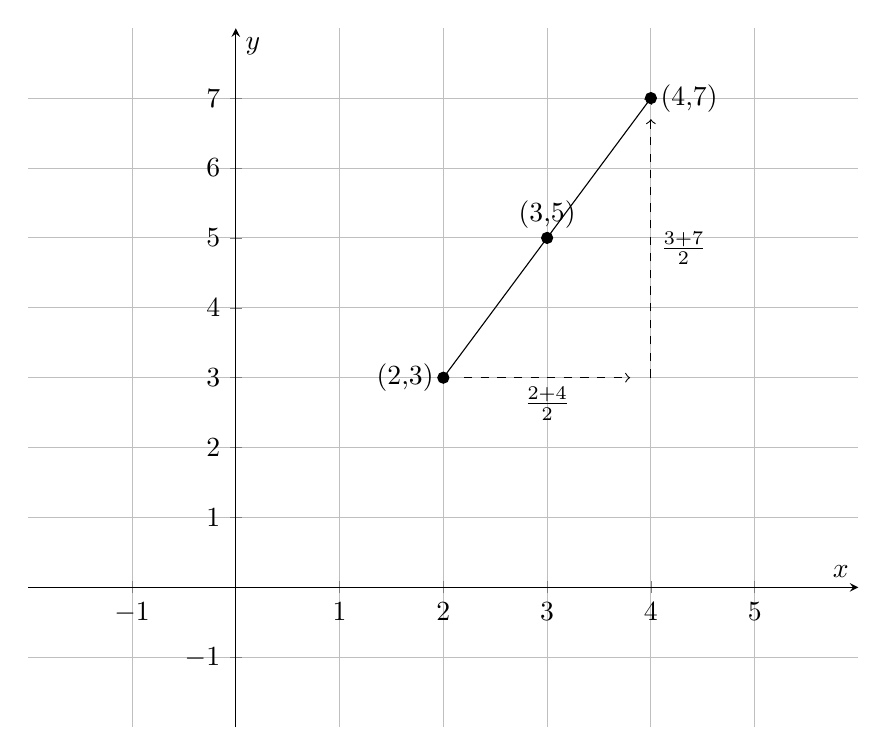
\begin{tikzpicture}
    \begin{axis}[width=\textwidth,
        axis lines = middle,
        xlabel = {$x$},
        ylabel = {$y$},
        ymin=-2, ymax=8,
        xmin=-2, xmax=6,
        ytick={-1,0,1,2,3,4,5,6,7},
        xtick={-1,0,1,2,3,4,5},
        grid=both,
        grid style={line width=.3pt, draw=gray!50}]
    \addplot [only marks, mark=*] coordinates {(2,3) (4,7) (3,5)};
    \draw[->] (axis cs:2,3) -- (axis cs:4,7);
    \node at (axis cs:2,3) [anchor=east] {(2,3)};
    \node at (axis cs:4,7) [anchor=west] {(4,7)};
    \node at (axis cs:3,5) [anchor=south] {(3,5)};
    \draw[->,dashed] (axis cs:2.2,3) -- (axis cs:3.8,3) node[midway, below] {$\frac{2+4}{2}$};
    \draw[->,dashed] (axis cs:4,3) -- (axis cs:4,6.7) node[midway, right] {$\frac{3+7}{2}$};
    \end{axis}
\end{tikzpicture}
\end{center}

\newpage

\section*{Equations of Perpendicular Lines}

Perpendicular means at a right angles with the horizon, or more generally it means any line that forms a right angle with another line. (In diagrams, this is denoted by a small square in the right angle.)\\

In algebra, two lines are perpendicular if the product of their slopes is \(-1\). If you have the equation of a line in slope-intercept form \(y = mx + b\), the slope of a line perpendicular to it will be \(-\frac{1}{m}\).\\

\subsection*{Example}

Given the line \(y = 2x + 3\), the slope is \(2\). Therefore, the slope of a line perpendicular to it is \(-\frac{1}{2}\).

\begin{center}
\begin{tikzpicture}
    \begin{axis}[width=\textwidth,
        axis lines = middle,
        xlabel = {$x$},
        ylabel = {$y$},
        ymin=-2, ymax=6,
        xmin=-6, xmax=5,
        domain=-5:5,
        samples=100,
        xtick={-5,-4,-3,-2,-1,0,1,2,3,4,5},
        ytick={-1,0,1,2,3,4,5},
        grid=both,
        grid style={line width=.3pt, draw=gray!50}
        ]
    \addplot [<->,domain=-2.2:1.2] {2*x + 3} node[pos=0.75, sloped, below] {$y=2x + 3$};
    \addplot [<->,domain=-4.5:4.5] {-0.5*x + 1} node[pos=0.2, sloped, above] {$y=-\frac{1}{2}x + 1$};
    \draw[fine] (-0.88,1.24) -- (-1.059,1.329) -- (-0.979,1.489);
    \end{axis}
\end{tikzpicture}
\end{center}

\newpage

\section*{Finding the Intersection Points of Two Lines}

To find the intersection point of two lines given by their equations, set the equations equal to each other and solve for \(x\) and \(y\).

\subsection*{Example}

Find the intersection of the lines \(y = 2x + 1\) and \(y = -x + 4\).

\[
2x + 1 = -x + 4
\]
\[
3x = 3 \implies x = 1
\]
\[
y = 2\cdot1 + 1 = 3
\]
The intersection point is \((1, 3)\).\\

\begin{center}
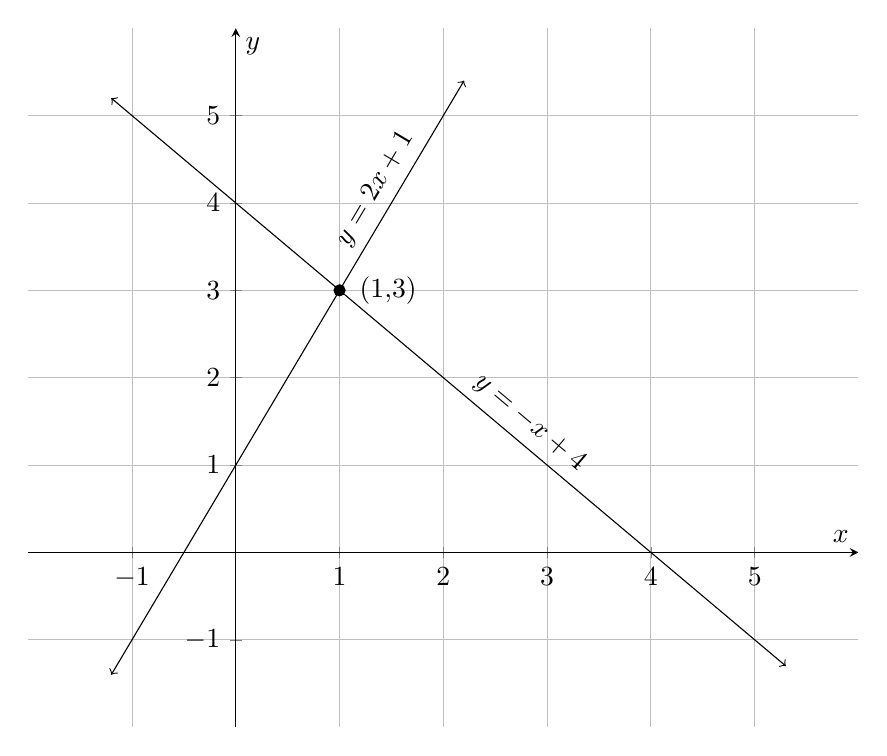
\begin{tikzpicture}
    \begin{axis}[width=\textwidth,
        axis lines = middle,
        xlabel = {$x$},
        ylabel = {$y$},
        ymin=-2, ymax=6,
        xmin=-2, xmax=6,
        domain=-2:6,
        samples=100,
        ytick={-1,0,1,2,3,4,5},
        xtick={-1,0,1,2,3,4,5},
        grid=both,
        grid style={line width=.3pt, draw=gray!50}]
    \addplot [<->,domain=-1.2:2.2] {2*x + 1} node[pos=0.8, above, sloped] {$y=2x+1$};
    \addplot [<->,domain=-1.2:5.3] {-x + 4} node[pos=0.6, above, sloped] {$y=-x+4$};
    \addplot [only marks, mark=*] coordinates {(1,3)};
    \node at (axis cs:1.1,3) [anchor=west] {(1,3)};
    \end{axis}
\end{tikzpicture}
\end{center}

\newpage

\section*{Exercises}

\subsection*{Finding the Length of a Line Segment}
\begin{enumerate}
    \item Find the distance between the points \((1, 2)\) and \((4, 6)\).
    \item Calculate the distance between the coordinates \((-3, -4)\) and \((3, 2)\).
    \item Determine the distance between the points \((0, 0)\) and \((5, 12)\).
\end{enumerate}

\subsection*{Finding the Midpoint of a Line Segment}
\begin{enumerate}
    \item Find the midpoint of the line segment with endpoints \((1, 2)\) and \((3, 6)\).
    \item Now plot those points on a set of axes, draw a line between them, meaure it, and mark the midpoint.
    
    Do these coordinates agree with the coordinates that you found algebraically?
    \item Find the midpoint of the line segment with endpoints \((0, 0)\) and \((4, 8)\).
    \item Plot these three points and check that the midpoint does in fact look like the midpoint.
\end{enumerate}

\subsection*{Equations of Perpendicular Lines}

\begin{enumerate}
    \item Find the equation of a line perpendicular to \(y = 3x - 2\).
    \item Plot these two lines to check that they are in fact perpendicular.
    \item What is the slope of a line perpendicular to the line \(y = -\frac{1}{4}x + 5\)?
\end{enumerate}

\subsection*{Finding the Intersection Points of Two Lines}
\begin{enumerate}
    \item Find the intersection point of the lines \(y = x + 2\) and \(y = -x + 4\).
    \item Plot these two lines and mark their point of intersection. Does this agree with your alebraic solution?
    \item Find the intersection of the lines \(y = 2x - 1\) and \(y = -\frac{1}{2}x + 3\).
    \item Plot these two lines and mark their point of intersection. Does this agree with your alebraic solution?
\end{enumerate}

\section*{Answers}

\subsection*{Finding the Length of a Line Segment}
\begin{enumerate}
    \item The distance between the points \((1, 2)\) and \((4, 6)\) is:
    \[
    d = \sqrt{(4 - 1)^2 + (6 - 2)^2} = \sqrt{3^2 + 4^2} = \sqrt{9 + 16} = \sqrt{25} = 5
    \]
    
    \item The distance between the points \((-3, -4)\) and \((3, 2)\) is:
    \[
    d = \sqrt{(3 - (-3))^2 + (2 - (-4))^2} = \sqrt{6^2 + 6^2} = \sqrt{36 + 36} = \sqrt{72} = 6\sqrt{2}
    \]
    
    \item The distance between the points \((0, 0)\) and \((5, 12)\) is:
    \[
    d = \sqrt{(5 - 0)^2 + (12 - 0)^2} = \sqrt{5^2 + 12^2} = \sqrt{25 + 144} = \sqrt{169} = 13
    \]
\end{enumerate}

\subsection*{Finding the Midpoint of a Line Segment}
\begin{enumerate}
    \item \((2, 4)\)
    \item \((2, 4)\)
\end{enumerate}

\subsection*{Equations of Perpendicular Lines}
\begin{enumerate}
    \item \(y = -\frac{1}{3}x + c\)
    \item The slope is \(4\).
\end{enumerate}

\subsection*{Finding the Intersection Points of Two Lines}
\begin{enumerate}
    \item \((1, 3)\)
    \item \((1.6, 2.2)\)
\end{enumerate}

\end{document}
